\chapter{Исследовательская часть}
В данном разделе будут выполнены сравнительный анализ двух методов решения задачи коммивояжера и параметризация метода на основе муравьиного алгоритма по трем его параметрам.

\section{Технические характеристики}
Характеристики используемого оборудования:
\begin{itemize}
    \item[---] операционная система --- Windows 11 Home [6];
    \item[---] память --- 16 Гб;
    \item[---] процессор --- Intel(R) Core(TM) i5-10300H CPU @ 2.50ГГц [7].
\end{itemize}

\section{Время выполнения алгоритмов}
Результаты замеров времени работы двух алгоритмов решения задачи коммивояжера приведены в таблице~\ref{tbl:time_measurements}. Время работы алгоритмов замерялось на указанном ранее оборудовании. Замеры времени проводились на матрицах одинаковой длины от 1 до 9 и усреднялись для каждого набора одинаковых серий замеров. Каждое значение получено путем взятия среднего из 40 измерений. Зависимости времени выполнения задачи от размера матрицы стоимостей для двух алгоритмов представлены на рисунке~\ref{fig:tm}.
\clearpage

\begin{table}[h]
	\begin{center}
		\begin{threeparttable}
		\captionsetup{justification=raggedright,singlelinecheck=off}
		\caption{Время работы алгоритмов (в мс)}
		\label{tbl:time_measurements}
		\begin{tabular}{|c|r|r|r|r|}
			\hline
			Размер матрицы &  Полный перебор & Муравьиный \\
            \hline
			1    & 0,115 & 0,863 \\
            \hline
			2    & 0,159 & 0,943 \\ 
            \hline
			3    & 0,081 & 0,948 \\ 
            \hline
			4    & 0,071 & 1,472 \\ 
			\hline
			5    & 0,952 & 2,460 \\ 
			\hline
			6    & 8,413 & 3,565 \\ 
			\hline
			7    & 85,019 & 4,527 \\ 
			\hline
			8    & 862,511 & 5,422 \\ 
			\hline
			9    & 11282,25 & 6,619 \\ 
            \hline
		\end{tabular}
		\end{threeparttable}
    \end{center}
\end{table}

\begin{figure}[h]
    \centering
    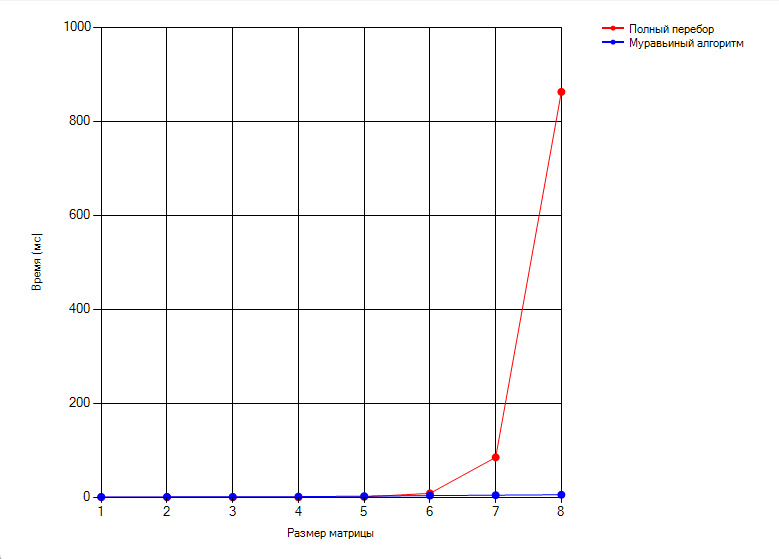
\includegraphics[width=0.8\linewidth]{img/graph-1.png}
    \caption{Сравнение алгоритмов по времени}
    \label{fig:tm}
\end{figure}

\section{Параметризация}

Целью проведения параметризации является определение таких комбинаций параметров, при которых муравьиный алгоритм дает наилучшие результаты.

В результате параметризации будет получена таблица со следующими столбцами:
\begin{itemize}
	\item[---] $a$ --- коэффициент влияния феромона;
    \item[---] $r$ --- коэффициент испарения феромона;
    \item[---] $t$ --- количество дней/итераций;
    \item[---] $mx, md, av$ --- максимальное, медианное и среднее арифметическое значение отклонения стоимости полученного марщрута от эталонного для каждого из трех графов.
\end{itemize}

\section{Класс данных}

Класс данных представляет собой набор из трех ориентированных графов, представленных в виде матриц стоимостей для 9 вершин:

\begin{equation}
    \mathbf{G_1} =
    \begin{pmatrix}
        0 & 10 & 15 & 20 & 25 & 30 & 35 & 40 & 45 \\
        12 & 0 & 37 & 27 & 19 & 26 & 33 & 18 & 17 \\
        14 & 35 & 0 & 32 & 22 & 23 & 28 & 24 & 26 \\
        16 & 29 & 30 & 0 & 33 & 17 & 27 & 28 & 31 \\
        18 & 21 & 24 & 35 & 0 & 37 & 32 & 20 & 23 \\
        20 & 31 & 29 & 19 & 31 & 0 & 22 & 26 & 29 \\
        22 & 33 & 34 & 25 & 28 & 24 & 0 & 22 & 25 \\
        24 & 23 & 26 & 27 & 22 & 29 & 26 & 0 & 13 \\
        26 & 25 & 28 & 29 & 25 & 31 & 29 & 15 & 0
    \end{pmatrix}
\end{equation}

\begin{equation}
    \mathbf{G_2} =
    \begin{pmatrix}
        0 & 12 & 18 & 24 & 30 & 36 & 42 & 48 & 54 \\
        14 & 0 & 23 & 29 & 35 & 41 & 47 & 53 & 59 \\
        16 & 25 & 0 & 38 & 44 & 50 & 56 & 62 & 68 \\
        18 & 27 & 40 & 0 & 53 & 59 & 65 & 71 & 77 \\
        20 & 29 & 42 & 55 & 0 & 68 & 74 & 80 & 86 \\
        22 & 31 & 44 & 57 & 70 & 0 & 83 & 89 & 95 \\
        24 & 33 & 46 & 59 & 72 & 85 & 0 & 98 & 104 \\
        26 & 35 & 48 & 61 & 74 & 87 & 96 & 0 & 110 \\
        28 & 37 & 50 & 63 & 76 & 89 & 102 & 115 & 0
    \end{pmatrix}
\end{equation}

\begin{equation}
    \mathbf{G_3} =
    \begin{pmatrix}
        0 & 14 & 20 & 18 & 24 & 32 & 40 & 26 & 22 \\
        16 & 0 & 24 & 30 & 36 & 40 & 44 & 28 & 20 \\
        18 & 26 & 0 & 28 & 32 & 36 & 40 & 30 & 22 \\
        20 & 28 & 30 & 0 & 38 & 42 & 46 & 32 & 24 \\
        22 & 30 & 34 & 40 & 0 & 48 & 52 & 34 & 26 \\
        24 & 32 & 36 & 42 & 48 & 0 & 56 & 36 & 28 \\
        26 & 34 & 38 & 44 & 50 & 56 & 0 & 38 & 30 \\
        28 & 36 & 40 & 46 & 52 & 58 & 64 & 0 & 18 \\
        30 & 38 & 42 & 48 & 54 & 60 & 66 & 18 & 0
    \end{pmatrix}
\end{equation}

Вырезка наилучших релультатов представлена в таблице~\ref{tbl:cut}.

\begin{table}[h]
\centering
\caption{Результаты параметризации (вырезка)}
\label{tbl:cut}
\begin{tabular}{|r|r|r|r|r|r|r|r|r|r|r|r|}
\hline
a & r & t & mxG1 & avG1 & mdG1 & mxG2 & avG2 & mdG2 & mxG3 & avG3 & mdG3 \\
\hline
0,5 & 0,3 & 50 & 3,00 & 0,90 & 0,00 & 6,00 & 5,10 & 6,00 & 4,00 & 2,80 & 2,00 \\
1 & 0,3 & 50 & 0,00 & 0,00 & 0,00 & 9,00 & 6,90 & 6,00 & 2,00 & 1,60 & 2,00 \\
1,5 & 0,3 & 50 & 0,00 & 0,00 & 0,00 & 9,00 & 7,50 & 7,50 & 4,00 & 2,60 & 2,00 \\
2 & 0,1 & 100 & 1,00 & 0,10 & 0,00 & 6,00 & 4,20 & 4,50 & 2,00 & 1,00 & 1,00 \\
2,5 & 0,1 & 100 & 0,00 & 0,00 & 0,00 & 9,00 & 6,60 & 6,00 & 2,00 & 1,80 & 2,00 \\
1 & 0,3 & 100 & 0,00 & 0,00 & 0,00 & 9,00 & 7,50 & 9,00 & 2,00 & 1,20 & 2,00 \\
1,5 & 0,3 & 100 & 0,00 & 0,00 & 0,00 & 12,00 & 6,90 & 9,00 & 6,00 & 3,20 & 2,00 \\
2 & 0,3 & 100 & 3,00 & 0,30 & 0,00 & 15,00 & 8,70 & 9,00 & 6,00 & 3,00 & 2,00 \\
2,5 & 0,3 & 250 & 3,00 & -0,90 & 0,00 & 15,00 & -21,00 & 6,00 & 6,00 & -1,60 & 2,00 \\
\hline
\end{tabular}
\end{table}

\clearpage

\section{Вывод}

В результате исследования было получено, что при $N < 7$ муравьиный алгоритм и алгоритм полного перебора выполянют задачу за примерно одинаковое время, а при $N\ge 7$ муравьиный алгоритм работает около в  раз быстрее, чем алгоритм полного перебора.

Также было выявлено, что при $a=2;r=0,1;t=100;$ муравьиный алгоритм дает наилучшие результаты.